% =============================================================================
% Chapter 7: Administration and Registration
% ניהול ואדמיניסטרציה
% NEW CHAPTER - Administrative processes and registration workflows
% =============================================================================

\documentclass[../master/main.tex]{subfiles}

\begin{document}

\setcounter{chapter}{6}
\hebrewchapter{ניהול ואדמיניסטרציה}
\hebrewchapterlabel{chap:administration}

\par\needspace{5\baselineskip}
\hebrewsection{מבוא --- שלושת רמות הרישום}

תהליך ההרשמה לפרויקט הגמר מתקיים בשלוש רמות נפרדות: רמת הסטודנט, רמת הקבוצה, ורמת סוכן ה-\en{AI}. הבנת ההבדלים בין הרמות חיונית להשלמת תהליך הרישום בהצלחה.

\needspace{10\baselineskip}
\begin{warningbox}[\hebtitle{שימו לב!!!}]
\textbf{כחלק מהתנהלות הפרויקט במהלך הפרויקט ובעיקר ערב או אפילו ביום קיום מחזור הליגה, יתכן והאדמיניסטרטור ישלח עדכוני מפרט או עדכוני פרוטוקול בצורת קובצי \en{PRD} בפורמט \en{MARKDOWN} שיהיה עליכם לעדכן בפרויקט שלכם. ההודעה תישלח בוואטסאפ של הקבוצה וגם דרך מנגנון שליחת ההודעות של המודל. מטרת הודעות אלו תהיה לוודא את גמישות הארכיטקטורה והקוד שלכם.}
\end{warningbox}

\par\needspace{4\baselineskip}
\hebrewsubsection{מטרות הפרק}

בסיום פרק זה, תדעו:
\begin{itemize}
    \item את תהליך הרישום המלא משלב בחירת הקבוצה ועד להפעלת הסוכנים
    \item את כללי בחירת שם הקבוצה ודרישות הפורמט
    \item כיצד להקים חשבונות \en{Gmail} עבור סוכני ה-\en{AI}
    \item כיצד להקים מאגרי קוד פרטיים ב-\en{GitHub}
    \item את כתובות האימייל של מנהל הליגה ושרת הלוגים
    \item כיצד להירשם במודל ולהגיש את קובץ ה-\en{PDF}
\end{itemize}

\par\needspace{4\baselineskip}
\hebrewsubsection{שלוש רמות הרישום}

\begin{enumerate}
    \item \textbf{רמת הסטודנט} --- כל סטודנט נרשם באופן אישי במודל באמצעות קובץ \en{PDF}
    \item \textbf{רמת הקבוצה} --- הקבוצה ממלאת טופס אלקטרוני משותף (מספיק חבר קבוצה אחד)
    \item \textbf{רמת הסוכן} --- שני סוכני \en{AI} (שחקן ושופט) נרשמים אוטומטית באמצעות הקוד
\end{enumerate}

איור~\ref{fig:registration-workflow} מציג את תהליך הרישום המלא.

\begin{figure}[htbp]
\centering
\begin{english}
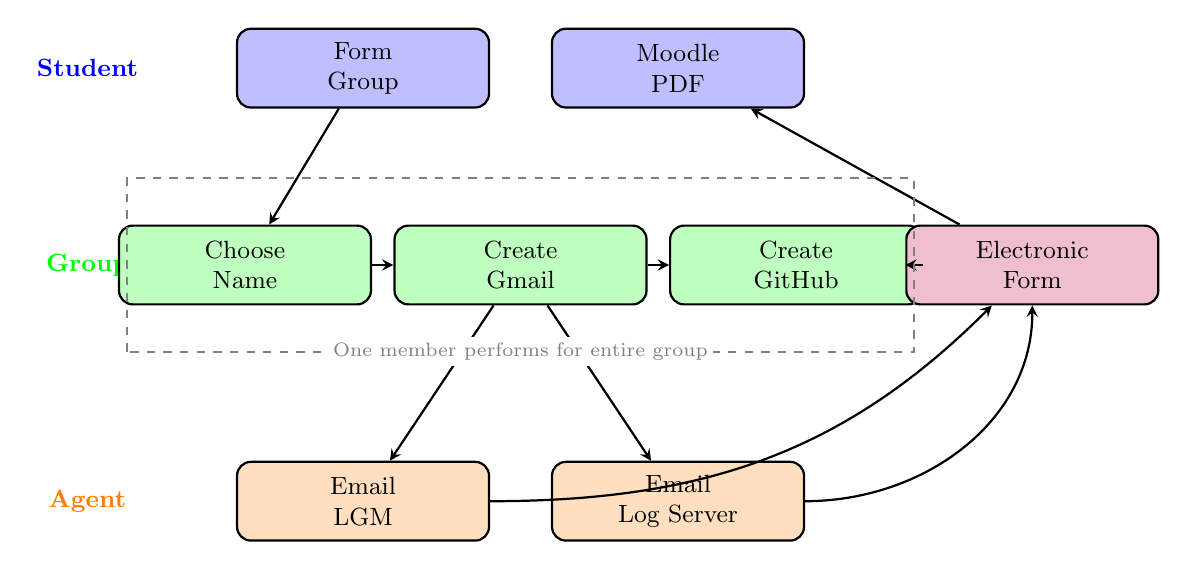
\begin{tikzpicture}[
    step/.style={draw, thick, fill=#1!25, minimum width=3.2cm, minimum height=1cm, rounded corners=5pt, align=center, font=\small},
    arrow/.style={->, thick, >=stealth},
    level/.style={font=\bfseries\small, text=#1}
]
    % Level labels
    \node[level=blue] at (-5.5,4) {Student};
    \node[level=green] at (-5.5,1.5) {Group};
    \node[level=orange] at (-5.5,-1.5) {Agent};

    % Student level
    \node[step=blue] (s1) at (-2,4) {Form\\Group};
    \node[step=blue] (s2) at (2,4) {Moodle\\PDF};

    % Group level
    \node[step=green] (g1) at (-3.5,1.5) {Choose\\Name};
    \node[step=green] (g2) at (0,1.5) {Create\\Gmail};
    \node[step=green] (g3) at (3.5,1.5) {Create\\GitHub};

    % Agent level
    \node[step=orange] (a1) at (-2,-1.5) {Email\\LGM};
    \node[step=orange] (a2) at (2,-1.5) {Email\\Log Server};

    % Form submission
    \node[step=purple] (form) at (6.5,1.5) {Electronic\\Form};

    % Arrows - horizontal at group level
    \draw[arrow] (s1) -- (g1);
    \draw[arrow] (g1) -- (g2);
    \draw[arrow] (g2) -- (g3);
    \draw[arrow] (g3) -- (form);

    % Arrows - vertical to agent level
    \draw[arrow] (g2) -- (a1);
    \draw[arrow] (g2) -- (a2);

    % Arrows - from agent to form (curved to avoid crossing text)
    \draw[arrow] (a1) to[out=0, in=-135] (form);
    \draw[arrow] (a2) to[out=0, in=-90] (form);

    % Arrow back to student level
    \draw[arrow] (form) -- (s2);

    % Dashed box around group level only
    \draw[dashed, thick, gray] (-5,0.4) rectangle (5,2.6);

    % Text below the dashed box, not crossing arrows
    \node[gray, font=\scriptsize, fill=white, inner sep=2pt] at (0,0.4) {One member performs for entire group};

\end{tikzpicture}
\end{english}
\caption{תהליך הרישום --- משלב בחירת הקבוצה ועד להגשה במודל}
\label{fig:registration-workflow}
\end{figure}

% =============================================================================
\par\needspace{5\baselineskip}
\hebrewsection{לוח זמנים מפורט}
\label{sec:calendar}
% =============================================================================

טבלה~\ref{tab:season-calendar} מציגה את לוח הזמנים המלא לשנת הלימודים הנוכחית.

\begin{fancytable}{lHcc}{לוח זמנים --- עונות הליגה}
\label{tab:season-calendar}
עונה & אירוע & תאריך & שעות \\
עונה א' & חימום מוקדם \en{1} & \en{Feb 3, 2026} & \en{18:30--21:00} \\
עונה א' & חימום מוקדם \en{2} & \en{Feb 10, 2026} & \en{18:30--21:00} \\
עונה א' & חימום מוקדם \en{3} & \en{Feb 16, 2026} & \en{18:30--21:00} \\
\textbf{עונה א'} & \textbf{ליגה} & \textbf{\en{Feb 17, 2026}} & \textbf{\en{18:30--22:00}} \\
עונה ב' & חימום מוקדם \en{1} & \en{Feb 24, 2026} & \en{18:30--21:00} \\
עונה ב' & חימום מוקדם \en{2} & \en{Mar 3, 2026} & \en{18:30--21:00} \\
עונה ב' & חימום מוקדם \en{3} & \en{Mar 16, 2026} & \en{18:30--21:00} \\
\textbf{עונה ב'} & \textbf{ליגה} & \textbf{\en{Mar 17, 2026}} & \textbf{\en{18:30--22:00}} \\
\end{fancytable}

\needspace{10\baselineskip}
\begin{notebox}[\hebtitle{תכנון מועדים}]
רשמו את המועדים הללו ביומן האישי שלכם. וודאו שאתם זמינים בכל חלון זמן של מחזור ליגה או חימום. היעדרות עלולה לגרום להפסד אוטומטי.
\end{notebox}

\needspace{10\baselineskip}
\begin{warningbox}[\hebtitle{הפעלה רציפה של הסוכנים}]
בכל עונה בה אתם רוצים שהסוכנים שלכם ישתתפו, הם צריכים לרוץ \textbf{באופן רציף}. הסוכנים צריכים לסרוק את חשבון ה-\en{Gmail} שלהם ולהיות מוכנים להגיב או לשלוח אימיילים בכל רגע. לדוגמה, במהלך עונת ליגה א' הסוכן צריך להיות פעיל במשך \num{3.5} שעות ברציפות.
\end{warningbox}

% =============================================================================
\par\needspace{5\baselineskip}
\hebrewsection{הקמת קבוצה}
\label{sec:group-formation}
% =============================================================================

\par\needspace{4\baselineskip}
\hebrewsubsection{בחירת חברי קבוצה}

\begin{itemize}
    \item \textbf{הרכב סטנדרטי} --- זוג סטודנטים בכל קבוצה
    \item \textbf{מקרים מיוחדים} --- באישור ראש המחלקה, המזכירות והמרצה:
    \begin{itemize}
        \item סטודנט יחיד בקבוצה
        \item שלושה סטודנטים בקבוצה (עם מטלות נוספות)
    \end{itemize}
\end{itemize}

\needspace{10\baselineskip}
\begin{notebox}[\hebtitle{המלצה}]
מומלץ מאוד למנות את אחד מחברי הקבוצה כ\textbf{אדמיניסטרטור} שאחראי על כל התהליכים הביורוקרטיים. זה יבטיח שכל השלבים יושלמו בצורה מסודרת.
\end{notebox}

\needspace{10\baselineskip}
\begin{warningbox}[\hebtitle{חובת זמינות}]
\textbf{כל חברי הקבוצה חייבים להיות זמינים} בכל חלון זמן של מחזור ליגה או מחזור חימום שהסוכן שלהם רשום אליו. היעדרות של אחד מחברי הקבוצה בזמן משחק פעיל עלולה לגרום להפסד אוטומטי ולפגיעה בציון הקבוצה. תכננו מראש את הזמינות שלכם לפני הרשמה לכל מחזור!
\end{warningbox}

\par\needspace{4\baselineskip}
\hebrewsubsection{כללי בחירת שם קבוצה}

שם הקבוצה חייב לעמוד בכל הדרישות הבאות:

\begin{enumerate}
    \item \textbf{אורך} --- בדיוק \num{8} תווים
    \item \textbf{תווים מותרים} --- אותיות קטנות באנגלית (\en{a-z}) וספרות (\en{0-9}) בלבד
    \item \textbf{תו פתיחה} --- חייב להתחיל באות (לא בספרה)
    \item \textbf{ללא רווחים} --- אסור לכלול רווחים או תווים מיוחדים
    \item \textbf{אנונימיות} --- אסור שיהיה ניתן לזהות את הסטודנטים לפי השם
    \item \textbf{ייחודיות} --- השם חייב להיות ייחודי במערכת
\end{enumerate}

\needspace{10\baselineskip}
\begin{warningbox}[\hebtitle{דרישת אנונימיות}]
שם הקבוצה \textbf{חייב להיות אנונימי}. אסור שהשם יכלול את שמותיכם האמיתיים, שמות משפחה, או כל מידע מזהה אחר. דרישה זו נועדה לשמור על פרטיות בטבלאות הליגה הפומביות. לדוגמאות נוספות ראו סעיף~\ref{sec:anonymous-names} בפרק~\ref{chap:overview}.
\end{warningbox}

טבלה~\ref{tab:group-name-examples} מציגה דוגמאות לשמות קבוצה חוקיים ולא חוקיים.

\begin{fancytable}{lHH}{דוגמאות לשמות קבוצה}
\label{tab:group-name-examples}
סוג & דוגמה & הסבר \\
חוקי & \en{bibi0707} & \num{8} תווים, מתחיל באות \\
חוקי & \en{agent123} & \num{8} תווים, אותיות וספרות \\
חוקי & \en{q21gteam} & \num{8} תווים, אותיות בלבד \\
\textbf{לא חוקי} & \en{team01} & רק \num{6} תווים \\
\textbf{לא חוקי} & \en{1234abcd} & מתחיל בספרה \\
\textbf{לא חוקי} & \en{yossi\_dan} & מכיל תו מיוחד \\
\textbf{לא חוקי} & \en{CohenLev} & מכיל אותיות גדולות \\
\end{fancytable}

% =============================================================================
\par\needspace{5\baselineskip}
\hebrewsection{הקמת חשבונות סוכני \en{AI}}
\label{sec:agent-accounts}
% =============================================================================

\par\needspace{4\baselineskip}
\hebrewsubsection{יצירת חשבונות \en{Gmail}}

כל קבוצה נדרשת לפתוח \textbf{שני חשבונות \en{Gmail} חדשים וחינמיים}:

\begin{enumerate}
    \item \textbf{חשבון לסוכן שחקן} --- לתקשורת של סוכן השחקן
    \item \textbf{חשבון לסוכן שופט} --- לתקשורת של סוכן השופט
\end{enumerate}

\needspace{10\baselineskip}
\begin{notebox}[\hebtitle{חובה \en{Gmail}}]
השימוש ב-\en{Gmail} הוא \textbf{חובה}. אין להשתמש בספקי דואר אלקטרוני אחרים. כל התקשורת במערכת מתבצעת באמצעות \en{Gmail API}. חשוב להכיר את מגבלות ה-\en{API} לפני המימוש --- ראו נספח~ה' לניתוח מפורט של מגבלות השליחה ומכסות ה-\en{API}.
\end{notebox}

\par\needspace{4\baselineskip}
\hebrewsubsection{פורמט כתובות הדואר האלקטרוני}

כתובות האימייל של הסוכנים חייבות לעקוב אחר הפורמט הבא:

\begin{itemize}
    \item \textbf{סוכן שחקן}: \texttt{\en{groupname.player@strudel.gmail.com}}
    \item \textbf{סוכן שופט}: \texttt{\en{groupname.referee@strudel.gmail.com}}
\end{itemize}

\needspace{10\baselineskip}
\begin{warningbox}[\hebtitle{דומיין \en{Strudel}}]
שימו לב לדומיין \texttt{\en{strudel.gmail.com}}. זהו דומיין מיוחד של מערכת הליגה. אסור להשתמש בכתובות \en{Gmail} רגילות.
\end{warningbox}

טבלה~\ref{tab:email-format} מציגה את פורמט כתובות האימייל עם דוגמאות.

\begin{fancytable}{lll}{פורמט כתובות אימייל לסוכנים}
\label{tab:email-format}
\en{Agent Type} & \en{Format} & \en{Example} \\
\en{Player} & \en{groupname.player@strudel.gmail.com} & \en{bibi0707.player@strudel.gmail.com} \\
\en{Referee} & \en{groupname.referee@strudel.gmail.com} & \en{bibi0707.referee@strudel.gmail.com} \\
\end{fancytable}

\par\needspace{4\baselineskip}
\hebrewsubsection{שליחת אימייל למנהל הליגה}

מיד לאחר פתיחת חשבונות ה-\en{Gmail}, יש לשלוח אימייל ידני למנהל הליגה:

\begin{enumerate}
    \item שלחו אימייל \textbf{מחשבון השחקן} לכתובת מנהל הליגה
    \item שלחו אימייל \textbf{מחשבון השופט} לכתובת מנהל הליגה
    \item המתינו לתשובה ממנהל הליגה לכל אחת מההודעות
\end{enumerate}

\needspace{12\baselineskip}
\begin{implementationbox}
כתובת מנהל הליגה: \texttt{\en{bitalevi100@gmail.com}}

ההרשמה תהיה מוכנה רק לאחר שתקבלו תשובה (\en{reply}) ממנהל הליגה לכל אחד מהאימיילים ששלחתם.
\end{implementationbox}

\par\needspace{4\baselineskip}
\hebrewsubsection{רישום פרוגרמטי לליגה}

לאחר הרישום הידני, הסוכן מבצע רישום אוטומטי בפורמט \en{JSON}:

\begin{english}
\begin{pythonbox}[\hebtitle{\en{LEAGUE\_REGISTER\_REQUEST}}]
{
  "message_type": "LEAGUE_REGISTER_REQUEST",
  "payload": {
    "agent_name": "bibi0707.player",
    "agent_type": "PLAYER",
    "email": "bibi0707.player@strudel.gmail.com",
    "group_name": "bibi0707",
    "version": "1.0"
  },
  "message_id": "uuid-v4",
  "timestamp": "2026-02-01T10:00:00Z"
}
\end{pythonbox}
\end{english}

השרת מחזיר \en{RESPONSE\_LEAGUE\_REGISTER} עם טבלת המשתמשים:

\begin{english}
\begin{pythonbox}[\hebtitle{\en{RESPONSE\_LEAGUE\_REGISTER}}]
{
  "message_type": "RESPONSE_LEAGUE_REGISTER",
  "payload": {
    "status": "REGISTERED",
    "agent_id": "P-bibi0707",
    "user_table": [
      {"agent_id": "P-bibi0707", "email": "bibi0707.player@..."},
      {"agent_id": "R-bibi0707", "email": "bibi0707.referee@..."},
      // ... more users
    ]
  },
  "correlation_id": "uuid-from-request"
}
\end{pythonbox}
\end{english}

\par\needspace{4\baselineskip}
\hebrewsubsection{רישום לעונה}

לאחר קבלת \en{BROADCAST\_SEASON\_START}, הסוכן נרשם לעונה:

\begin{english}
\begin{pythonbox}[\hebtitle{\en{SEASON\_REGISTRATION\_REQUEST}}]
{
  "message_type": "SEASON_REGISTRATION_REQUEST",
  "payload": {
    "agent_id": "P-bibi0707",
    "season_id": "S01"
  },
  "message_id": "uuid-v4",
  "timestamp": "2026-02-01T12:00:00Z"
}
\end{pythonbox}
\end{english}

\begin{warningbox}[\hebtitle{חלון רישום סוכנים}]
רישום סוכן לעונה מתבצע באופן \textbf{אוטונומי} בתחילת ערב הליגה:
\begin{itemize}
    \item \textbf{חלון רישום}: \en{18:30--18:45} (\num{15} דקות)
    \item \textbf{טריגר}: הודעת \en{BROADCAST\_START\_SEASON} או אירוע \en{REG\_SEASON} ביומן המשותף
    \item \textbf{תוצאה}: הסוכן נרשם אוטומטית לעונה הנוכחית
\end{itemize}
לאחר \en{18:45}, חלון הרישום נסגר ולא ניתן להירשם לעונה הנוכחית.
\end{warningbox}

\begin{notebox}[\hebtitle{הבחנה בין סוגי רישום}]
\textbf{רישום קבוצה/משתמש} (\en{Manual Registration}): מתבצע חד-פעמית על ידי הסטודנטים באמצעות טופס אלקטרוני ו-\en{PDF} במודל.

\textbf{רישום סוכן לעונה} (\en{Autonomous Registration}): מתבצע באופן אוטונומי על ידי הסוכנים בתחילת כל ערב ליגה.
\end{notebox}

\par\needspace{4\baselineskip}
\hebrewsubsection{מניעת ספאם}

כדי למנוע בעיות ספאם משני הכיוונים, יש לבצע את הפעולות הבאות:

\begin{enumerate}
    \item בכל חשבון \en{Gmail} של סוכן, היכנסו לרשימת אנשי הקשר (\en{Contacts})
    \item הוסיפו את כתובת מנהל הליגה: \texttt{\en{bitalevi100@gmail.com}}
    \item הוסיפו את כתובת שרת הלוגים: \texttt{\en{beit.halevi.700@gmail.com}}
    \item שמרו את אנשי הקשר
\end{enumerate}

\needspace{10\baselineskip}
\begin{warningbox}[\hebtitle{חשוב מאוד}]
ללא הוספת מנהל הליגה לרשימת אנשי הקשר, הודעות הברודקאסט של המערכת עלולות להיחסם כספאם. בנוסף, הודעות שתשלחו עלולות להיחשב כספאם על ידי \en{Google}. לאסטרטגיות מניעה נוספות והמלצות למימוש, ראו נספח~ה' סעיף~\ref{sec:spam-risks}.
\end{warningbox}

\par\needspace{10\baselineskip}
\hebrewsubsection{חובת סריקת תיקיית ספאם}

\needspace{6\baselineskip}
\begin{protocolbox}
בנוסף להוספת אנשי קשר, \textbf{כל סוכן (שחקן ושופט) חייב לסרוק את תיקיית הספאם} בשלבים הראשוניים של התקשורת. דרישה זו חלה גם על מנהל הליגה.
\end{protocolbox}

\textbf{מתי לסרוק?}
\begin{itemize}
    \item מיד לאחר שליחת אימייל הרישום הידני --- לבדוק אם התשובה הגיעה לספאם
    \item בתחילת כל משחק --- לפני שלב החימום
    \item בכל פעם שלא מתקבלת תגובה צפויה בזמן
\end{itemize}

\needspace{10\baselineskip}
\begin{notebox}[\hebtitle{פרטים נוספים}]
לפרטים מלאים על דרישת סריקת הספאם וההמלצות למימוש, ראו סעיף~\ref{sec:spam-scanning} בפרק~\ref{chap:protocol}.
\end{notebox}

% =============================================================================
\par\needspace{5\baselineskip}
\hebrewsection{הקמת מאגרי קוד ב-\en{GitHub}}
\label{sec:github-setup}
% =============================================================================

\par\needspace{4\baselineskip}
\hebrewsubsection{יצירת ריפוזיטורי פרטי}

בשונה ממטלות הבית, מאגרי הקוד של פרויקט הגמר \textbf{חייבים להיות פרטיים} (\en{Private}):

\begin{enumerate}
    \item צרו ריפוזיטורי פרטי עבור \textbf{סוכן השחקן}
    \item צרו ריפוזיטורי פרטי עבור \textbf{סוכן השופט}
    \item בשלב הראשוני, מספיק ליצור קובץ \en{README} בלבד
\end{enumerate}

\needspace{10\baselineskip}
\begin{notebox}[\hebtitle{פרטיות הקוד}]
הריפוזיטורי חייב להיות \en{Private} ולא \en{Public}. זאת מכיוון שהקוד שלכם מהווה חלק מההגשה ואינו אמור להיות נגיש לקבוצות אחרות.
\end{notebox}

\par\needspace{4\baselineskip}
\hebrewsubsection{הוספת שותף עריכה}

כדי שמנהל הליגה יוכל לבדוק את הקוד ולתת ציון, יש להוסיף אותו כשותף:

\needspace{12\baselineskip}
\begin{implementationbox}
\textbf{שלבי הוספת שותף ב-\en{GitHub}:}

\begin{enumerate}
    \item היכנסו לריפוזיטורי ב-\en{GitHub}
    \item לחצו על \en{Settings} (בפינה הימנית העליונה)
    \item בתפריט הצד, בחרו \en{Collaborators} תחת \en{Access}
    \item לחצו על \en{Add people}
    \item הזינו את הכתובת: \texttt{\en{bitalevi100@gmail.com}}
    \item שלחו את ההזמנה
    \item מנהל הליגה יאשר את ההזמנה
\end{enumerate}

חזרו על התהליך עבור שני הריפוזיטורים (שחקן ושופט).
\end{implementationbox}

% =============================================================================
\par\needspace{5\baselineskip}
\hebrewsection{הרשמה לשרת הלוגים}
\label{sec:log-server}
% =============================================================================

בנוסף לשליחת אימייל למנהל הליגה, יש לשלוח אימייל גם לשרת הלוגים:

\begin{enumerate}
    \item שלחו אימייל ידני \textbf{מחשבון השחקן} לשרת הלוגים
    \item שלחו אימייל ידני \textbf{מחשבון השופט} לשרת הלוגים
    \item הוסיפו את שרת הלוגים לרשימת אנשי הקשר בשני החשבונות
\end{enumerate}

\needspace{10\baselineskip}
\begin{implementationbox}
כתובת שרת הלוגים: \texttt{\en{beit.halevi.700@gmail.com}}

שרת הלוגים מקבל העתק (\en{CC}) של כל ההודעות במהלך המשחקים. זה מאפשר תיעוד, ביקורת, ויישוב מחלוקות במקרה הצורך.
\end{implementationbox}

% =============================================================================
\par\needspace{5\baselineskip}
\hebrewsection{רישום במודל}
\label{sec:moodle-registration}
% =============================================================================

\par\needspace{4\baselineskip}
\hebrewsubsection{עקרונות הרישום}

להלן הנחיות הרישום לפרויקט הגמר בקורס אורכסטרציית סוכני \en{AI}:

\begin{enumerate}
    \item כל סטודנט, \textbf{באופן אישי}, חייב להירשם דרך מטלת פרויקט הגמר במודל
    \item כל סטודנט הוא חבר בקבוצה
    \item כל סטודנט נרשם לקבוצה על ידי הגשת קובץ \en{PDF} הכולל את כל השדות הנדרשים
\end{enumerate}

\par\needspace{4\baselineskip}
\hebrewsubsection{מילוי הטופס האלקטרוני לרישום סוכנים}

לאחר השלמת כל השלבים הקודמים, יש למלא את הטופס האלקטרוני לרישום סוכני ה-\en{AI} של הקבוצה לליגה:

\begin{enumerate}
    \item היכנסו למודל ופתחו את מטלת פרויקט הגמר
    \item מצאו את הקישור לטופס רישום סוכני \en{AI} לליגה: \\ \url{https://docs.google.com/forms/d/e/1FAIpQLSe2EZJ7k-61S-Qtl2JVYK12uI2246LPTxzVRwAgNJC8--0-fg/viewform}
    \item מלאו את כל השדות הנדרשים (שם קבוצה, כתובות אימייל של הסוכנים, קישורים לריפוזיטורים)
    \item אשרו ששלחתם אימיילים למנהל הליגה ולשרת הלוגים
    \item שלחו את הטופס
\end{enumerate}

\needspace{10\baselineskip}
\begin{notebox}[\hebtitle{טופס אחד לקבוצה}]
מספיק שחבר קבוצה \textbf{אחד} ימלא את הטופס האלקטרוני לרישום סוכני ה-\en{AI} לליגה. הטופס מייצג את רישום הסוכנים של הקבוצה כולה.
\end{notebox}

\par\needspace{4\baselineskip}
\hebrewsubsection{הגשת קובץ \en{PDF} אישי}

בשונה מהטופס האלקטרוני, \textbf{כל סטודנט חייב להירשם במודל באופן אישי} על ידי הגשת קובץ \en{PDF}.

\textbf{השדות הנדרשים בקובץ ה-\en{PDF}:}

\begin{enumerate}
    \item \textbf{שם הקבוצה} --- שם הקבוצה בן \num{8} התווים שבחרתם
    \item \textbf{פרטי חברי הקבוצה} --- עבור \textbf{כל} חבר קבוצה יש לציין:
    \begin{enumerate}
        \item שם פרטי
        \item שם משפחה
        \item מספר תעודת זהות
    \end{enumerate}
    \item \textbf{פרטי סוכן השופט (\en{Referee Agent})}:
    \begin{enumerate}
        \item כתובת האימייל של הסוכן (בפורמט \en{groupname.referee@gmail.com})
        \item קישור לריפוזיטורי ה-\en{GitHub} של הסוכן
    \end{enumerate}
    \item \textbf{פרטי סוכן השחקן (\en{Player Agent})}:
    \begin{enumerate}
        \item כתובת האימייל של הסוכן (בפורמט \en{groupname.player@gmail.com})
        \item קישור לריפוזיטורי ה-\en{GitHub} של הסוכן
    \end{enumerate}
\end{enumerate}

\begin{fancytable}{lH}{שדות קובץ ה-\en{PDF} לרישום}
\label{tab:pdf-fields}
קטגוריה & שדות נדרשים \\
פרטי קבוצה & שם קבוצה (\num{8} תווים) \\
פרטי כל חבר & שם פרטי, שם משפחה, תעודת זהות \\
סוכן שופט & כתובת אימייל, קישור ל-\en{GitHub} \\
סוכן שחקן & כתובת אימייל, קישור ל-\en{GitHub} \\
\end{fancytable}

\needspace{10\baselineskip}
\begin{warningbox}[\hebtitle{חובת הגשה אישית}]
ההגשה במודל היא \textbf{אישית} ולא קבוצתית. כל סטודנט חייב להגיש בנפרד כדי שיוכל לקבל ציון. סטודנט שלא יגיש לא יוכל לקבל ציון על פרויקט הגמר.
\end{warningbox}

% =============================================================================
\par\needspace{5\baselineskip}
\hebrewsection{ספר כתובות המערכת}
\label{sec:contact-directory}
% =============================================================================

טבלה~\ref{tab:system-contacts} מרכזת את כל כתובות האימייל החשובות במערכת.

{\small
\begin{fancytable}{llH}{ספר כתובות המערכת}
\label{tab:system-contacts}
\en{Role} & \en{Email Address} & תפקיד \\
\en{League Manager (LGM)} & \en{bitalevi100@gmail.com} & רישום, ניהול משחקים, ציונים \\
\en{Log Server} & \en{beit.halevi.700@gmail.com} & תיעוד, \en{CC} בהודעות המשחק \\
\en{Player Agent} & \en{groupname.player@strudel.gmail.com} & תקשורת סוכן השחקן \\
\en{Referee Agent} & \en{groupname.referee@strudel.gmail.com} & תקשורת סוכן השופט \\
\end{fancytable}
}

\needspace{10\baselineskip}
\begin{notebox}[\hebtitle{שמות סוכנים במערכת}]
שמות הסוכנים במערכת נגזרים משם הקבוצה:
\begin{itemize}
    \item \textbf{סוכן שחקן}: \texttt{\en{groupname.player}} (לדוגמה: \en{MyGroup.player})
    \item \textbf{סוכן שופט}: \texttt{\en{groupname.referee}} (לדוגמה: \en{MyGroup.referee})
\end{itemize}
\end{notebox}

% =============================================================================
\par\needspace{5\baselineskip}
\hebrewsection{מדריך כתובות האימייל המלא}
\label{sec:email-directory}
% =============================================================================

סעיף זה מרכז את \textbf{כל} כתובות האימייל המופיעות בספר זה, כולל כתובות המערכת, דפוסי כתובות הסוכנים, וכתובות יצירת קשר.

\par\needspace{4\baselineskip}
\hebrewsubsection{כתובות מערכת קבועות}

\begin{fancytable}{lHH}{כתובות מערכת קבועות}
\label{tab:system-emails}
\en{Email} & בעלים & תפקיד \\
\en{bitalevi100@gmail.com} & מנהל הליגה (\en{LGM}) & רישום, ניהול משחקים, ציונים \\
\en{beit.halevi.700@gmail.com} & שרת הלוגים & \en{CC} בהודעות, תיעוד \\
\en{yoram.segal@post.runi.ac.il} & ד"ר יורם סגל & מרצה, מנהל ראשי \\
\end{fancytable}

\par\needspace{4\baselineskip}
\hebrewsubsection{דפוסי כתובות סוכנים}

\begin{fancytable}{lHH}{דפוסי כתובות סוכנים (לפי שם קבוצה)}
\label{tab:agent-email-patterns}
\en{Email Pattern} & סוג סוכן & תפקיד \\
\en{groupname.player@strudel.gmail.com} & סוכן שחקן & שאלות וניחושים \\
\en{groupname.referee@strudel.gmail.com} & סוכן שופט & רמזים וציונים \\
\end{fancytable}

\par\needspace{4\baselineskip}
\hebrewsubsection{כתובות גנריות לתיעוד בקוד}

\begin{fancytable}{lHH}{כתובות גנריות (לתיעוד בקוד)}
\label{tab:generic-emails}
\en{Symbolic Address} & משמעות & להחליף ב- \\
\en{league.manager@gmail.com} & מנהל הליגה & \en{bitalevi100@gmail.com} \\
\en{log.server@gmail.com} & שרת הלוגים & \en{beit.halevi.700@gmail.com} \\
\end{fancytable}

\needspace{10\baselineskip}
\begin{notebox}[\hebtitle{הבהרה חשובה}]
\begin{itemize}
    \item \textbf{כתובות קבועות}: הכתובות \en{bitalevi100@gmail.com} ו-\en{beit.halevi.700@gmail.com} הן הכתובות \textbf{בפועל} שיש להשתמש בהן.
    \item \textbf{דפוסי כתובות}: החליפו את \en{groupname} בשם הקבוצה שלכם (לדוגמה: \en{bibi0707.player@gmail.com}).
    \item \textbf{כתובות גנריות}: משמשות לתיעוד בקוד ובקבצי תצורה, ויש להחליפן בכתובות הממשיות.
    \item \textbf{פנייה למרצה}: לשאלות אקדמיות ומנהליות, פנו לד"ר יורם סגל בכתובת \en{yoram.segal@post.runi.ac.il}.
\end{itemize}
\end{notebox}

\par\needspace{4\baselineskip}
\hebrewsubsection{סיכום כתובות לפי תפקיד}

{\small
\begin{fancytable}{HlH}{כתובות לפי תפקיד}
\label{tab:emails-by-role}
תפקיד & כתובת & מתי להשתמש \\
מרצה הקורס & \en{yoram.segal@post.runi.ac.il} & שאלות אקדמיות, ערעורים \\
מנהל הליגה & \en{bitalevi100@gmail.com} & רישום, משחקים, ציונים \\
שרת הלוגים & \en{beit.halevi.700@gmail.com} & \en{CC} בכל הודעה \\
סוכן שחקן & \en{groupname.player@strudel.gmail.com} & תקשורת במשחקים \\
סוכן שופט & \en{groupname.referee@strudel.gmail.com} & תקשורת במשחקים \\
\end{fancytable}
}

% =============================================================================
\par\needspace{5\baselineskip}
\hebrewsection{רשימת בדיקה לסטודנט}
\label{sec:checklist}
% =============================================================================

להלן רשימת הבדיקה המלאה לתהליך הרישום. סמנו כל שלב לאחר השלמתו:

\begin{enumerate}
    \item[$\square$] \textbf{בחירת קבוצה} --- מצאתי שותף/ים לקבוצה
    \item[$\square$] \textbf{בחירת שם} --- בחרנו שם קבוצה בן \num{8} תווים, אנונימי וייחודי
    \item[$\square$] \textbf{חשבון שחקן} --- פתחתי חשבון \en{Gmail} חדש עבור סוכן השחקן בפורמט \en{groupname.player@gmail.com}
    \item[$\square$] \textbf{חשבון שופט} --- פתחתי חשבון \en{Gmail} חדש עבור סוכן השופט בפורמט \en{groupname.referee@gmail.com}
    \item[$\square$] \textbf{אימייל למנהל (שחקן)} --- שלחתי אימייל למנהל הליגה מחשבון השחקן
    \item[$\square$] \textbf{אימייל למנהל (שופט)} --- שלחתי אימייל למנהל הליגה מחשבון השופט
    \item[$\square$] \textbf{תשובה מהמנהל} --- קיבלתי תשובה ממנהל הליגה לשני האימיילים
    \item[$\square$] \textbf{אנשי קשר} --- הוספתי את מנהל הליגה ושרת הלוגים לאנשי הקשר בשני החשבונות
    \item[$\square$] \textbf{ריפוזיטורי שחקן} --- יצרתי ריפוזיטורי פרטי ריק עבור סוכן השחקן, עם קובץ \en{README} לפחות
    \item[$\square$] \textbf{ריפוזיטורי שופט} --- יצרתי ריפוזיטורי פרטי ריק עבור סוכן השופט, עם קובץ \en{README} לפחות
    \item[$\square$] \textbf{שותף עריכה} --- הוספתי את מנהל הליגה כשותף עריכה בשני הריפוזיטורים
    \item[$\square$] \textbf{אימייל ללוג (שחקן)} --- שלחתי אימייל לשרת הלוגים מחשבון השחקן
    \item[$\square$] \textbf{אימייל ללוג (שופט)} --- שלחתי אימייל לשרת הלוגים מחשבון השופט
    \item[$\square$] \textbf{סריקת ספאם} --- בדקתי את תיקיית הספאם בשני החשבונות לוודא שלא הגיעו הודעות לשם
    \item[$\square$] \textbf{טופס אלקטרוני} --- מילאתי (או חבר הקבוצה מילא) את הטופס האלקטרוני לרישום \num{2} סוכני \en{AI} לליגת \en{Q21G}
    \item[$\square$] \textbf{רישום ביומן} --- רשמתי ביומן האישי את חלונות הזמן לאימון הסוכנים ואת מועדי מחזורי הליגה
    \item[$\square$] \textbf{הגשה במודל} --- הגשתי את קובץ ה-\en{PDF} האישי במודל הכולל את פרטי חברי הקבוצה וסוכני ה-\en{AI}. \textbf{חובה}: כל סטודנט נרשם בנפרד במודל
\end{enumerate}

\needspace{10\baselineskip}
\begin{notebox}[\hebtitle{סיום ההרשמה}]
לאחר השלמת כל השלבים ברשימת הבדיקה, אתם מוכנים להתחיל בפיתוח הסוכנים. זכרו שברגע שהליגה נפתחת, הסוכנים נרשמים אוטומטית באמצעות הקוד שתכתבו --- כל מה שעשיתם כאן הוא הכנה ידנית חד-פעמית.
\end{notebox}

\end{document}
